% =====================================================================================
%  Energy Market Intelligence System — final project presentation
%  Compile with pdfLaTeX (Overleaf: Menu -> Compiler -> pdfLaTeX). Main file: main.tex
%  Self-contained: every image lives under ./figures/ (relative paths). No shell-escape.
%  Figures are produced by figures.py (run locally; see README.md).
% =====================================================================================
\documentclass[aspectratio=169,11pt]{beamer}

% ---- packages (all standard / Overleaf-safe) ----------------------------------------
\usepackage[T1]{fontenc}
\usepackage[utf8]{inputenc}
\usepackage{textcomp}                 % \texteuro
\usepackage{lmodern}
\usepackage{microtype}
\usepackage{graphicx}
\usepackage{booktabs}
\usepackage{array}
\usepackage{xcolor}
\usepackage{tikz}
\usetikzlibrary{arrows.meta,positioning,calc,fit,backgrounds,shapes.geometric}
\usepackage{pgfplots}\pgfplotsset{compat=1.18}
\usepackage{amsmath,amssymb}
\usepackage{ragged2e}

% ---- palette (mirrors figures.py exactly) -------------------------------------------
\definecolor{emisInk}{HTML}{1A2331}
\definecolor{emisMuted}{HTML}{5B6573}
\definecolor{emisGrid}{HTML}{D9DEE5}
\definecolor{emisAccent}{HTML}{0E7C86}   % data / global teal
\definecolor{modImp}{HTML}{7A5195}        % imputation / SSHB
\definecolor{modA}{HTML}{2C7FB8}          % load
\definecolor{modB}{HTML}{D9772B}          % price
\definecolor{modC}{HTML}{2E8B57}          % RL dispatch
\definecolor{emisGood}{HTML}{2E8B57}
\definecolor{emisWarn}{HTML}{E0A800}
\definecolor{emisBad}{HTML}{C0392B}

% ---- theme: clean custom (no nav bar -> maximum usable height) ----------------------
\usetheme{default}
\setbeamertemplate{navigation symbols}{}
\setbeamercolor{normal text}{fg=emisInk}
\setbeamercolor{structure}{fg=emisAccent}
\setbeamerfont{frametitle}{size=\Large,series=\bfseries}
\setlength{\parskip}{2pt}

% current "act" name + accent colour (set by \setact, drives title rule + footer)
\newcommand{\actname}{}
\newcommand{\actcolor}{emisAccent}
\newcommand{\setact}[2]{\renewcommand{\actname}{#1}\renewcommand{\actcolor}{#2}}

\setbeamertemplate{frametitle}{%
  \vskip0.5em%
  {\usebeamerfont{frametitle}\color{emisInk}\insertframetitle\par}%
  \vskip2pt%
  {\color{\actcolor}\rule{\textwidth}{1.1pt}}%
}
\setbeamertemplate{footline}{%
  \hbox to\paperwidth{\hskip2.2ex
    {\color{\actcolor}\footnotesize\bfseries\actname}\hfill
    {\color{emisMuted}\scriptsize Energy Market Intelligence System}\hfill
    {\color{emisMuted}\footnotesize\insertframenumber}\hskip2.2ex}%
  \vskip2.4pt%
}
\setbeamertemplate{itemize item}{\color{\actcolor}\small\textbullet}
\setbeamertemplate{itemize subitem}{\color{\actcolor}\scriptsize\textendash}

% ---- helper macros ------------------------------------------------------------------
\newcommand{\eur}{\texteuro}
\newcommand{\fig}[1]{\centering\includegraphics[width=\linewidth,height=0.62\textheight,keepaspectratio]{#1}}
\newcommand{\figbig}[1]{\centering\includegraphics[width=\linewidth,height=0.78\textheight,keepaspectratio]{#1}}
\newcommand{\cap}[1]{\\[2pt]{\footnotesize\color{emisMuted} #1}}
% stat card for the closing slide
\newcommand{\statcard}[3]{% colour, big, small
  \colorbox{#1!12}{\parbox[t][2.4cm][c]{0.30\textwidth}{\centering
    {\Large\bfseries\color{#1} #2}\\[3pt]{\footnotesize\color{emisInk} #3}}}}

\tikzset{
  emisbox/.style={rounded corners=3pt, draw, line width=1pt, align=center,
                  minimum height=1.0cm, inner sep=4pt, font=\small\bfseries, text=emisInk},
  qarr/.style={-{Stealth[length=2.6mm]}, line width=1pt},
  emisnote/.style={font=\scriptsize\itshape, text=emisMuted, align=center},
}

% q10/q50/q90 "fan of uncertainty" motif
\newcommand{\qfan}[1][1.0]{%
\begin{tikzpicture}[scale=#1]
  \fill[modB!16] (0,0) -- (4,0.95) -- (4,-0.95) -- cycle;
  \draw[modB!55, line width=1pt] (0,0) -- (4,0.95) node[right,font=\scriptsize\bfseries,text=modB]{q90};
  \draw[modB!55, line width=1pt] (0,0) -- (4,-0.95) node[right,font=\scriptsize\bfseries,text=modB]{q10};
  \draw[modB, line width=1.4pt] (0,0) -- (4,0) node[right,font=\scriptsize\bfseries,text=modB]{q50};
  \node[font=\scriptsize, text=emisMuted] at (1.0,-1.25) {forecast horizon $\rightarrow$};
\end{tikzpicture}}

% ---- metadata -----------------------------------------------------------------------
\title{Energy Market Intelligence System}
\date{June 2026}

\begin{document}

% =====================================================================================
% 1 — TITLE
% =====================================================================================
\begin{frame}[plain]
  \centering
  \vspace{0.5cm}
  {\color{emisAccent}\rule{0.66\textwidth}{1.2pt}}\\[0.45cm]
  {\LARGE\bfseries\color{emisInk} Energy Market Intelligence System}\\[0.30cm]
  {\large\color{emisMuted} Forecasting and battery dispatch \emph{under uncertainty}\\[2pt]
   in the German--Luxembourg day-ahead electricity market}\\[0.55cm]
  \qfan[0.78]\\[0.55cm]
  % >>> EDIT: replace the bracketed placeholder with the real team members <<<
  {\small\color{emisInk} \textbf{[\,Team member 1 \quad$\cdot$\quad Team member 2 \quad$\cdot$\quad Team member 3\,]}}\\[0.10cm]
  {\footnotesize\color{emisMuted} Free University of Bozen-Bolzano \;$\cdot$\; M.Sc.\ \;$\cdot$\; Machine Learning project \;$\cdot$\; June 2026}
  \vspace{0.3cm}
  \note{Welcome — 15 minutes, mixed audience, kept visual.
  One idea ties everything together: \emph{uncertainty propagation}. Three ML modules,
  each forecasting a band (q10/q50/q90), feeding the next. Set timing: ~45 s here.}
\end{frame}

% =====================================================================================
% 2 — THE PROBLEM
% =====================================================================================
\setact{Uncertainty propagation}{emisAccent}
\begin{frame}{Day-ahead prices are hard to predict}
  \begin{itemize}\setlength\itemsep{2pt}
    \item Spikes to \eur543/MWh, prices going \emph{negative} to $-$\eur236/MWh.
    \item Volatile, regime-shifting --- a single point forecast is fragile.
  \end{itemize}
  \vspace{2pt}
  \centering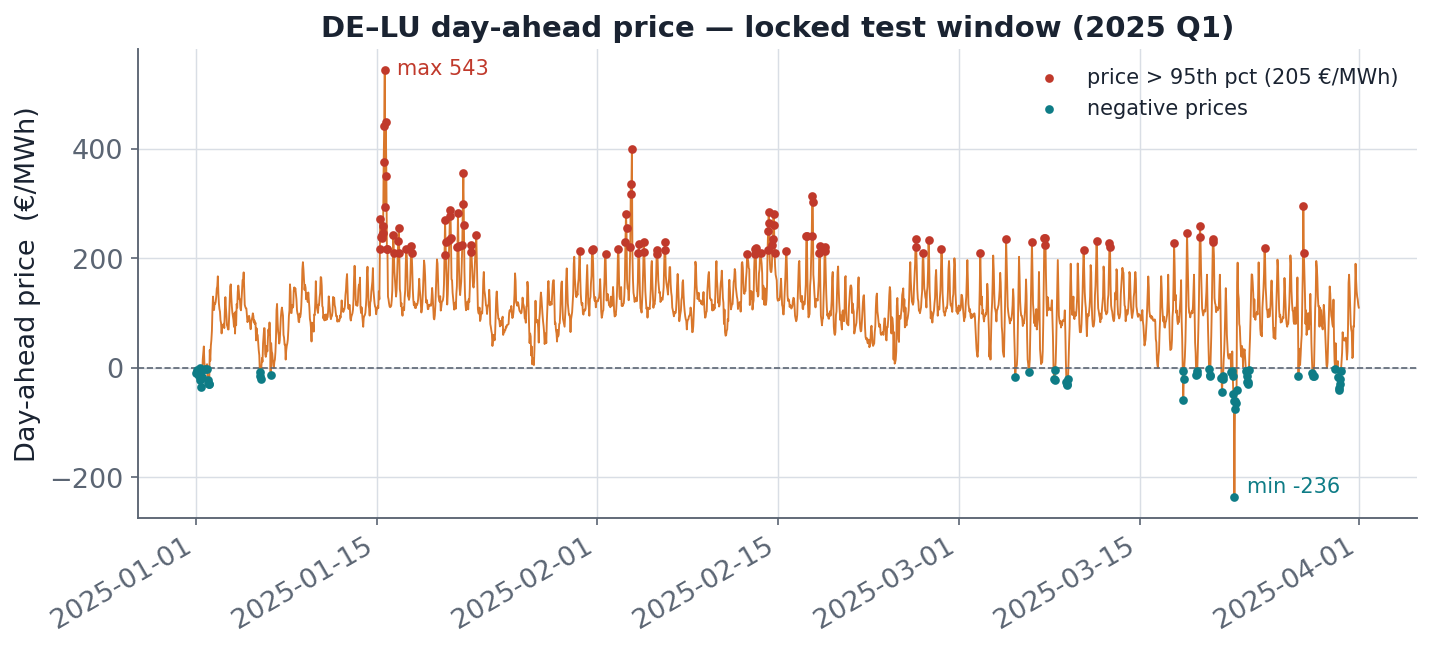
\includegraphics[width=\linewidth,height=0.56\textheight,keepaspectratio]{figures/raw_price_volatility.png}
  \note{Motivation. The German--Luxembourg spot price is spiky and shifts regime.
  Renewables and gas swings push it from negative to extreme highs. Point forecasts
  break exactly when decisions matter most. ~45 s.}
\end{frame}

% =====================================================================================
% 3 — THESIS
% =====================================================================================
\begin{frame}{Our answer: forecast the band, not the point}
  \begin{columns}[T,onlytextwidth]
    \begin{column}{0.50\textwidth}
      \small
      \begin{itemize}\setlength\itemsep{6pt}
        \item Every stage predicts \textbf{q10 / q50 / q90}, not one number.
        \item That uncertainty is \textbf{propagated} to the next stage.
        \item The final stage turns the band into \textbf{euros}.
      \end{itemize}
    \end{column}
    \begin{column}{0.48\textwidth}
      \centering\qfan[0.95]
    \end{column}
  \end{columns}
  \vspace{0.35cm}
  \begin{center}
    \colorbox{emisAccent!10}{\parbox{0.92\textwidth}{\centering\itshape
      ``Every stage admits what it doesn't know --- and that propagated
       uncertainty is what ultimately turns a battery into profit.''}}
  \end{center}
  \note{The thesis. We never claim a single true price. We quantify uncertainty as
  quantiles and carry it forward. Say the quoted sentence aloud — it is the through-line
  for the whole talk. ~45 s.}
\end{frame}

% =====================================================================================
% 4 — ARCHITECTURE
% =====================================================================================
\setact{Architecture}{emisAccent}
\begin{frame}{One pipeline, five stages}
  \vspace{0.2cm}
  \resizebox{\textwidth}{!}{%
  \begin{tikzpicture}[node distance=6mm]
    \node[emisbox, draw=emisAccent, fill=emisAccent!10] (data) at (0,0) {External\\data APIs};
    \node[emisbox, draw=modImp, fill=modImp!12] (sshb) at (3.1,0) {SSHB\\imputation};
    \node[emisbox, draw=emisMuted, fill=emisGrid!55] (clean) at (6.2,0) {Clean hourly\\data + splits};
    \node[emisbox, draw=modA, fill=modA!12] (A) at (9.6,1.5) {Module A\\Load $\cdot$ LSTM};
    \node[emisbox, draw=modB, fill=modB!14] (B) at (9.6,-1.5) {Module B\\Price $\cdot$ CatBoost};
    \node[emisbox, draw=modC, fill=modC!14] (C) at (13.1,0) {Module C\\RL dispatch};
    \node[emisbox, draw=emisInk, fill=emisGrid!35, minimum width=1.7cm] (out) at (16.0,0) {Battery\\schedule (\eur)};
    \draw[qarr, draw=emisAccent] (data)--(sshb);
    \draw[qarr, draw=modImp] (sshb)--(clean);
    \draw[qarr, draw=emisMuted] (clean.east) to[out=10,in=180] (A.west);
    \draw[qarr, draw=emisMuted] (clean.east) to[out=-10,in=180] (B.west);
    \draw[qarr, draw=modA] (A.east) to[out=0,in=120] node[above,sloped,font=\scriptsize\bfseries,text=modA]{load q10/q50/q90} (C.north west);
    \draw[qarr, draw=modB] (B.east) to[out=0,in=-120] node[below,sloped,font=\scriptsize\bfseries,text=modB]{price q10/q50/q90} (C.south west);
    \draw[qarr, draw=modC] (C)--(out);
  \end{tikzpicture}}
  \vspace{0.25cm}
  \begin{center}{\footnotesize\color{emisMuted}
   Raw data is repaired once, then two forecasters and one decision agent each consume the previous stage's \emph{quantiles}.}\end{center}
  \note{The map. Read left to right: ingest, repair missing values with SSHB, build
  fixed train/val/test splits, then Module A (load) and Module B (price) each emit
  quantiles, and Module C consumes them to schedule a battery. I'll walk this chain
  stage by stage; the footer tells you where we are. ~50 s.}
\end{frame}

% =====================================================================================
% 5 — DATA SOURCES
% =====================================================================================
\setact{Data}{emisAccent}
\begin{frame}{Six external data sources}
  \centering
  \footnotesize
  \begin{tabular}{@{}l l l@{}}
    \toprule
    \textbf{Source} & \textbf{Signal} & \textbf{Endpoint / note}\\
    \midrule
    ENTSO-E & Day-ahead price (\eur/MWh) & A44 (market zone)\\
    ENTSO-E & Actual load (MW) & A65 (physical zone)\\
    ENTSO-E & Generation, 17 fuels (MW) & A75\\
    ENTSO-E & Cross-border flows FR/AT/CH & A11\\
    Open-Meteo & Weather, 5 German cities & temp, wind, radiation\\
    Yahoo / Energy-Charts & TTF gas \& EU-ETS carbon & daily fuel prices\\
    \bottomrule
  \end{tabular}
  \vspace{0.35cm}
  \begin{itemize}\setlength\itemsep{2pt}
    \item Hourly, 2019--2025 \;$\approx$\; \textbf{61{,}368} rows, 47 raw $\rightarrow$ 52 columns.
    \item Two EIC codes (market vs.\ physical zone) --- using the wrong one returns empty.
  \end{itemize}
  \note{Data. Four ENTSO-E endpoints plus weather and fuels. Don't read the table —
  point at the three families: market (price), system (load/generation/flows), and
  drivers (weather, gas, carbon). Two EIC codes is the classic gotcha. ~40 s.}
\end{frame}

% =====================================================================================
% 6 — MISSINGNESS
% =====================================================================================
\begin{frame}{Missing data is structured, not random}
  \begin{columns}[T,onlytextwidth]
    \begin{column}{0.40\textwidth}
      \small
      \begin{itemize}\setlength\itemsep{6pt}
        \item Coal-gas: \emph{no} ENTSO-E data for 2019--2022.
        \item Nuclear $\rightarrow$ 0 after the 2023-04-15 shutdown.
        \item Plus scattered holiday / exchange gaps.
      \end{itemize}
      \vspace{4pt}
      {\footnotesize\color{emisMuted} A naïve fill would inject fake signal --- so we impute carefully.}
    \end{column}
    \begin{column}{0.58\textwidth}
      \centering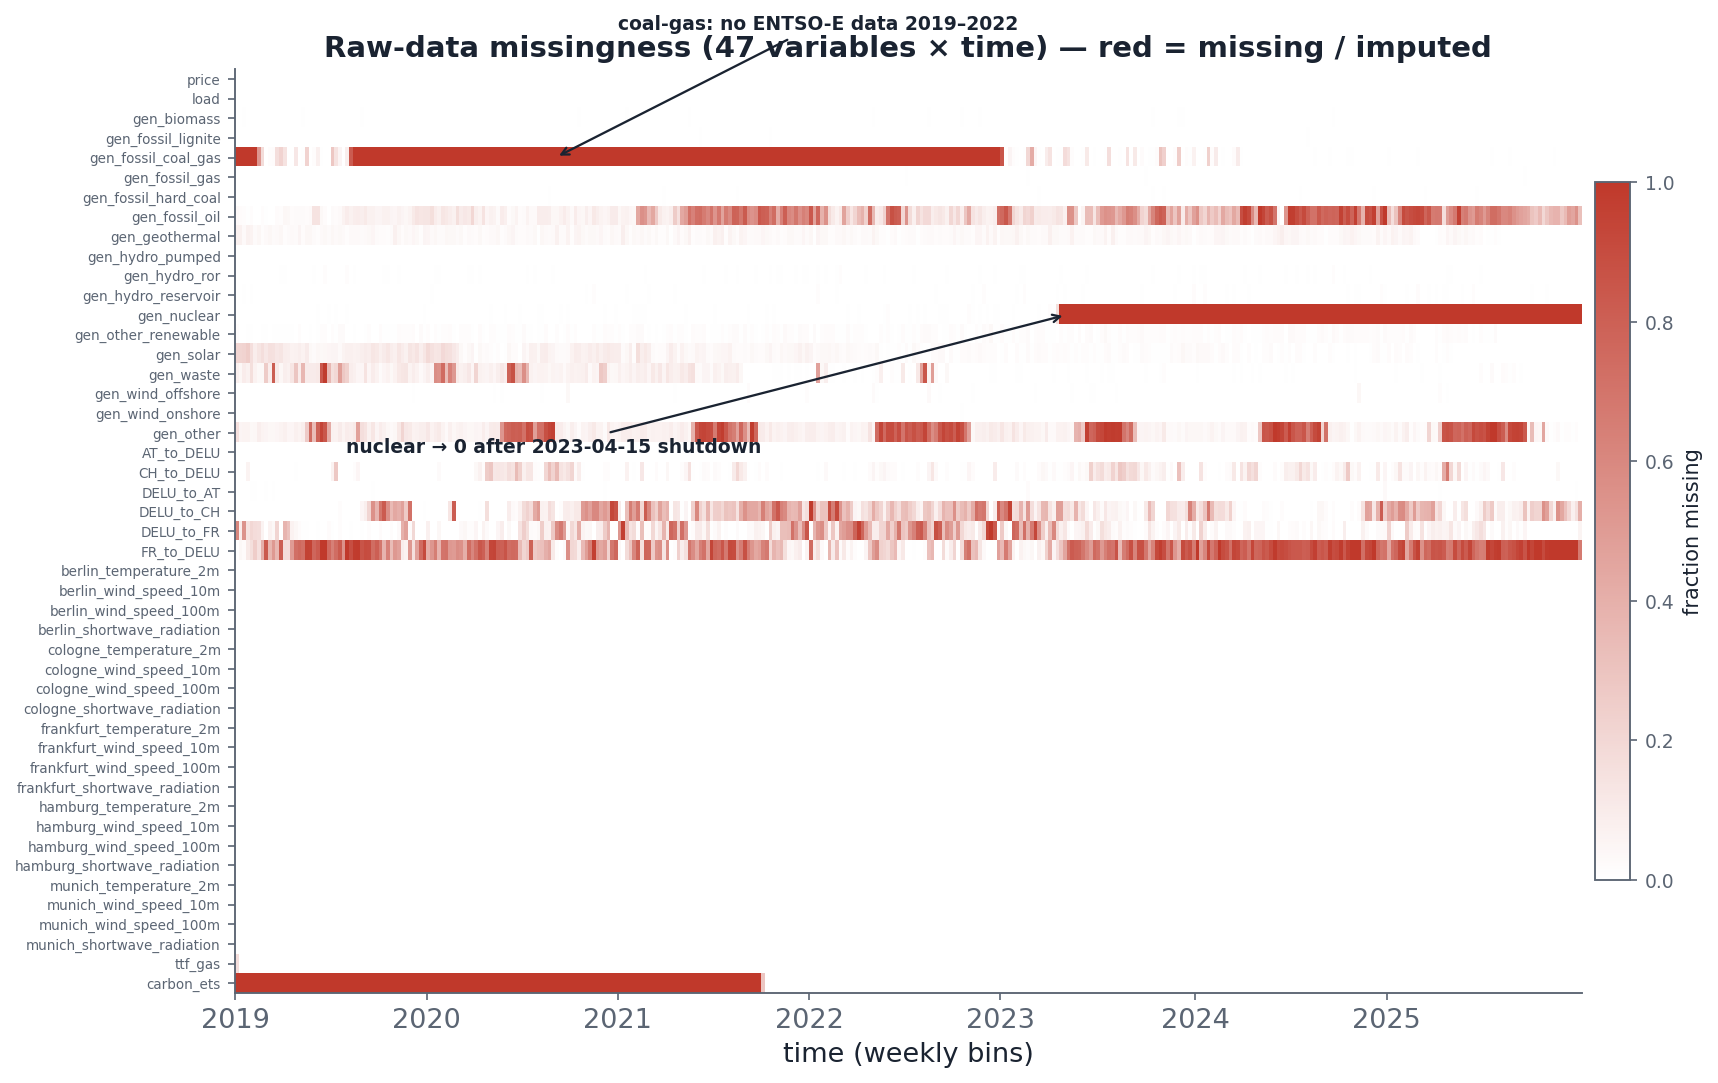
\includegraphics[width=\linewidth,height=0.78\textheight,keepaspectratio]{figures/missingness_heatmap.png}
    \end{column}
  \end{columns}
  \note{Why imputation matters. The red blocks are systematic, not random: a structural
  hole in coal-gas, the nuclear phase-out, holiday gaps. Filling these wrong would poison
  every downstream model — so the imputer has to be principled. ~45 s.}
\end{frame}

% =====================================================================================
% 7 — SSHB MECHANISM
% =====================================================================================
\setact{Imputation (SSHB)}{modImp}
\begin{frame}{SSHB --- self-supervised held-out blend}
  \vspace{0.1cm}
  \resizebox{\textwidth}{!}{%
  \begin{tikzpicture}[node distance=6mm]
    \node[emisbox, draw=emisMuted, fill=emisGrid!55] (obs) at (0,0) {Observed\\series};
    \node[emisbox, draw=emisMuted, fill=emisGrid!40] (mask) at (3.4,0) {Masked\\input};
    \node[emisbox, draw=modImp, fill=modImp!14] (md) at (7.2,1.35) {SAITS deep\\model \;(A)};
    \node[emisbox, draw=emisMuted, fill=emisGrid!55] (sm) at (7.2,-1.35) {Whittaker--Henderson\\smoother \;(B)};
    \node[emisbox, draw=modImp, fill=modImp!22] (blend) at (11.2,0) {Blend $w_i^{\star}$\\per feature};
    \node[emisbox, draw=emisInk, fill=emisGrid!40] (out) at (14.7,0) {Impute the\\missing cells};
    \draw[qarr, draw=emisMuted] (obs)-- node[above,font=\scriptsize\bfseries,text=emisInk]{hold out 10\%} (mask);
    \draw[qarr, draw=modImp] (mask.east) to[out=20,in=180] (md.west);
    \draw[qarr, draw=emisMuted] (mask.east) to[out=-20,in=180] (sm.west);
    \draw[qarr, draw=modImp] (md.east) to[out=0,in=120] (blend.north west);
    \draw[qarr, draw=emisMuted] (sm.east) to[out=0,in=-120] (blend.south west);
    \draw[qarr, draw=modImp] (blend)--(out);
  \end{tikzpicture}}
  \vspace{0.15cm}
  \begin{columns}[T,onlytextwidth]
    \begin{column}{0.97\textwidth}\small
      \begin{itemize}\setlength\itemsep{2pt}
        \item Held-out \emph{observed} cells pick the model/smoother blend per feature --- \textbf{no test labels touched}.
        \item Deep model = SAITS\,(Glocal-IB fork), transformer over 168-h windows; \textbf{observed values never overwritten}.
      \end{itemize}
    \end{column}
  \end{columns}
  \note{The imputer. SSHB is inference-time. We deliberately hide 10\% of the cells we
  actually observe, ask both a deep transformer and a smoother to predict them, and let
  the held-out cells vote on the blend per feature. Self-supervised because the
  ``answers'' are real observed values, not test data. ~55 s.}
\end{frame}

% =====================================================================================
% 8 — SSHB RESULTS
% =====================================================================================
\begin{frame}{SSHB improves quality with zero regressions}
  \begin{columns}[T,onlytextwidth]
    \begin{column}{0.56\textwidth}
      \centering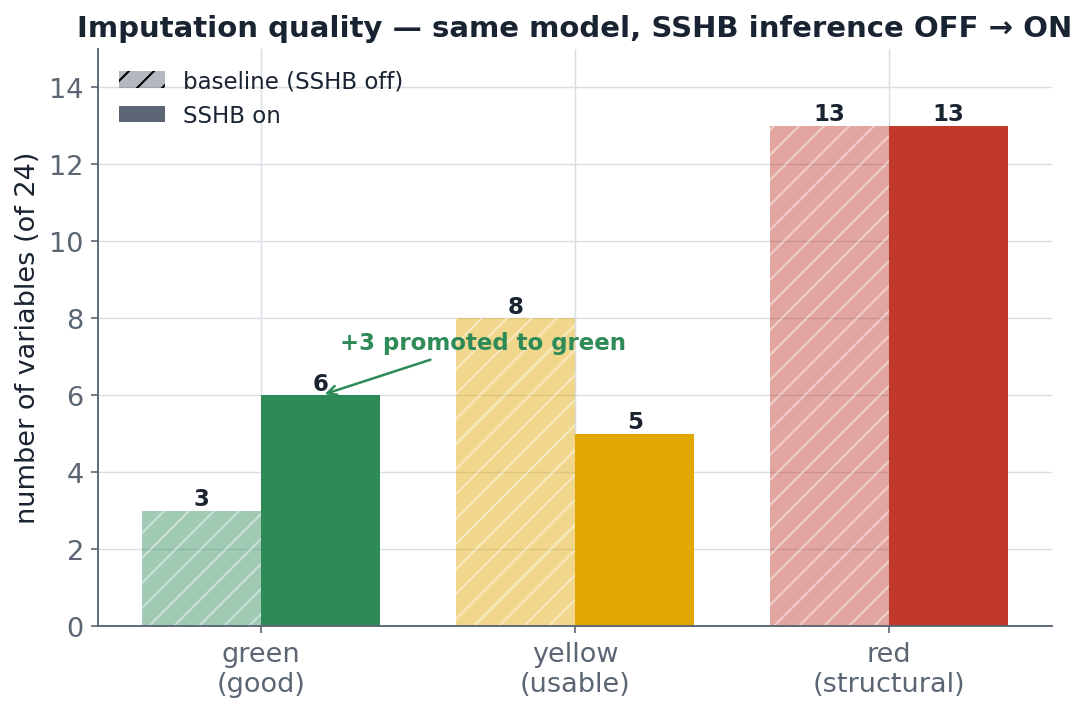
\includegraphics[width=\linewidth,height=0.74\textheight,keepaspectratio]{figures/sshb_audit_status.png}
    \end{column}
    \begin{column}{0.42\textwidth}
      \small
      \begin{itemize}\setlength\itemsep{7pt}
        \item Engages \textbf{53.9\%} of imputed cells.
        \item \textbf{+3} variables promoted to ``green''.
        \item \textbf{0} physical violations --- no regressions.
        \item Distribution match improves (std-ratio error 0.57$\to$0.55).
      \end{itemize}
    \end{column}
  \end{columns}
  \note{Result. Toggling SSHB on the same trained model promotes three variables from
  usable to good, engages over half the imputed cells, and introduces zero physical
  violations. Honest framing: 13 variables stay structurally red — we cannot invent data
  that the API never had. ~50 s.}
\end{frame}

% =====================================================================================
% 9 — MODULE A MODEL
% =====================================================================================
\setact{Module A --- Load}{modA}
\begin{frame}{Module A --- multi-scale load forecasting}
  \begin{columns}[T,onlytextwidth]
    \begin{column}{0.42\textwidth}
      \small
      \begin{itemize}\setlength\itemsep{6pt}
        \item Dual-branch LSTM: \textbf{48 h} + \textbf{168 h} history.
        \item Shared head $\rightarrow$ q10/q50/q90 for h1--24.
        \item Trained with \textbf{pinball loss}; calibrated by CQR.
      \end{itemize}
      \vspace{3pt}
      {\footnotesize\color{emisMuted} The first quantile emitter in the chain.}
    \end{column}
    \begin{column}{0.56\textwidth}
      \centering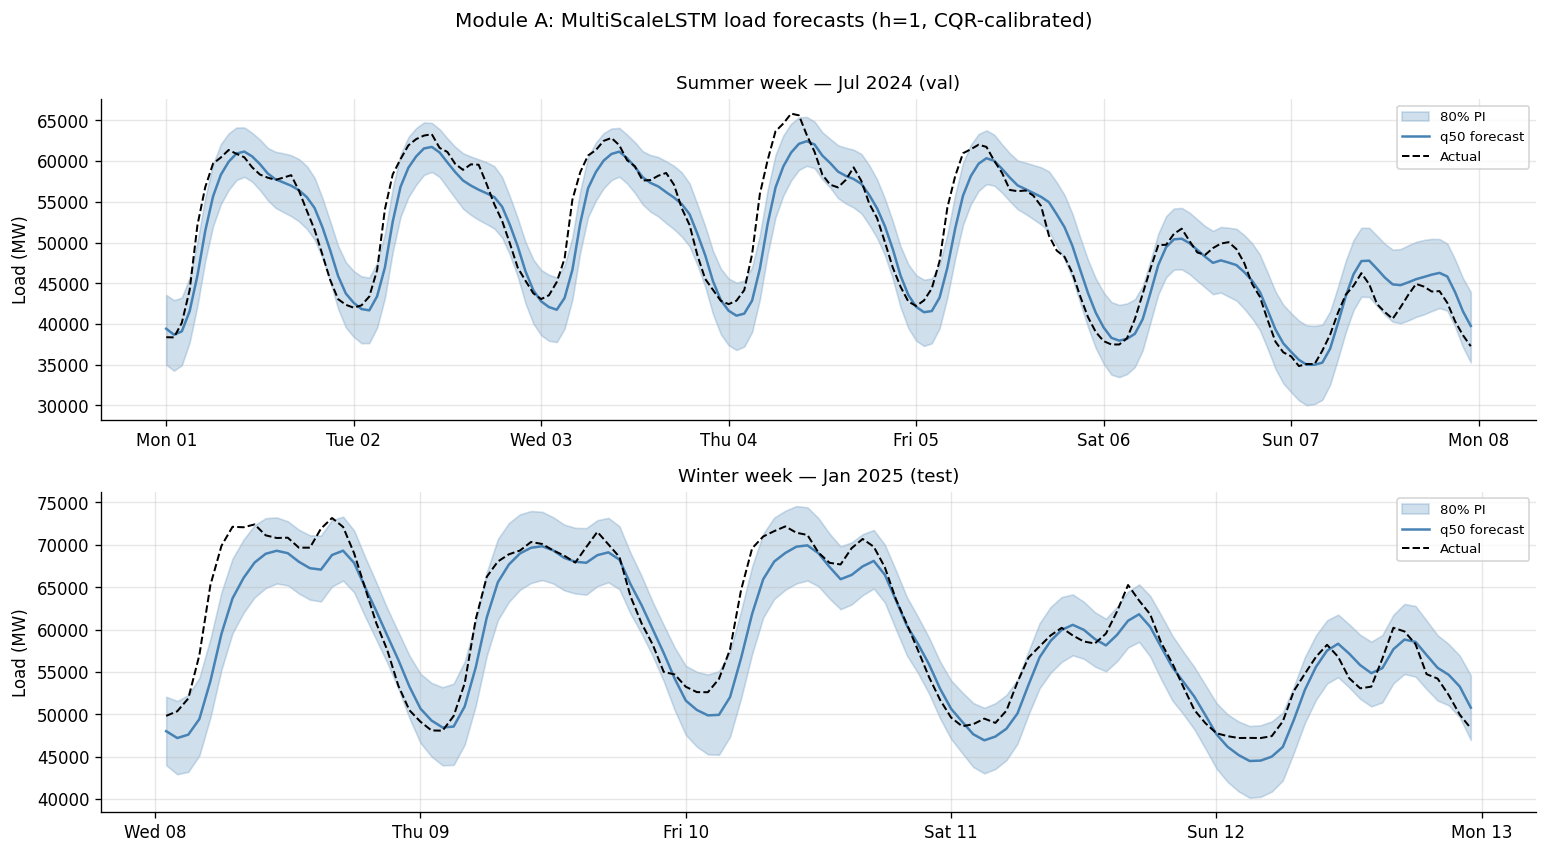
\includegraphics[width=\linewidth,height=0.74\textheight,keepaspectratio]{figures/module_a_sample_weeks.png}
    \end{column}
  \end{columns}
  \note{Module A. Two LSTM branches capture daily and weekly rhythm; the head outputs a
  full quantile fan for the next 24 hours. The plot shows summer and winter sample weeks —
  the shaded band is the 80\% interval tracking actual load. ~45 s.}
\end{frame}

% =====================================================================================
% 10 — MODULE A RESULTS
% =====================================================================================
\begin{frame}{Calibrated load intervals}
  \begin{columns}[T,onlytextwidth]
    \begin{column}{0.58\textwidth}
      \centering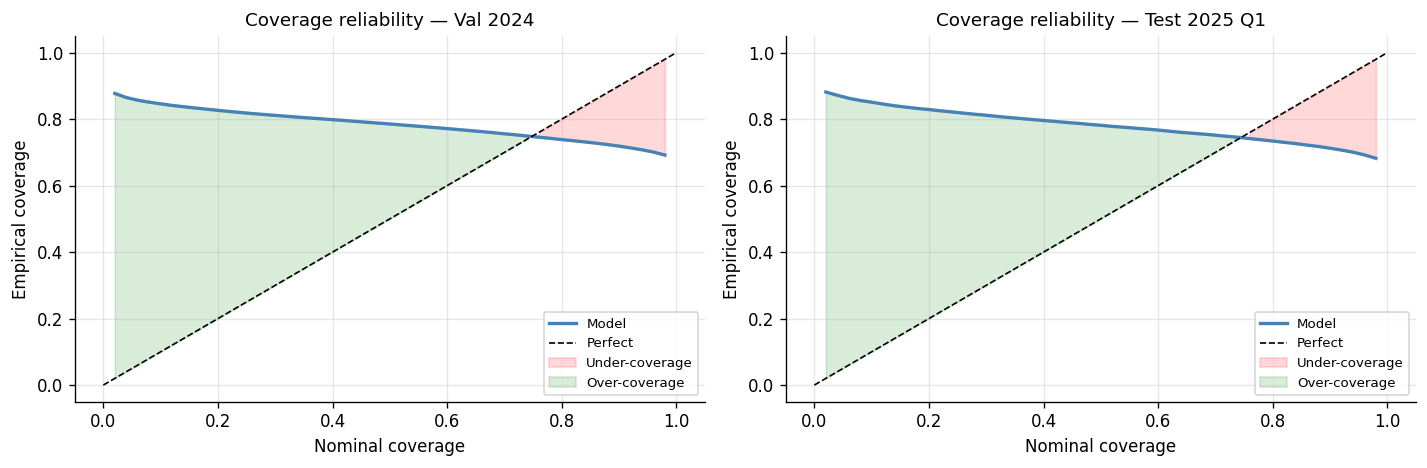
\includegraphics[width=\linewidth,height=0.72\textheight,keepaspectratio]{figures/module_a_reliability.png}
    \end{column}
    \begin{column}{0.40\textwidth}
      \small
      \begin{itemize}\setlength\itemsep{7pt}
        \item q50 MAE \textbf{2{,}591 MW} ($\approx$ 5\% nMAE).
        \item Beats the 1-week seasonal-naive baseline.
        \item CQR widens the band ($\delta$ \textbf{+1{,}596 MW}) to restore $\approx$80\% coverage.
      \end{itemize}
    \end{column}
  \end{columns}
  \note{Calibration. The raw model is mildly mis-calibrated (reliability curve off the
  diagonal). Conformal Quantile Regression adds a data-driven margin so the 80\% band
  actually covers 80\%. Same idea reused in Module B. ~45 s.}
\end{frame}

% =====================================================================================
% 11 — MODULE B MODEL
% =====================================================================================
\setact{Module B --- Price}{modB}
\begin{frame}{Module B --- price forecasting (production)}
  \begin{columns}[T,onlytextwidth]
    \begin{column}{0.50\textwidth}
      \small
      \begin{itemize}\setlength\itemsep{6pt}
        \item \textbf{Three independent} CatBoost quantile boosters (q10/q50/q90).
        \item $\approx$33 features, all strictly \textbf{past-only} (causal).
        \item Per-quantile depth \& regularisation tuned for the tails.
      \end{itemize}
    \end{column}
    \begin{column}{0.48\textwidth}
      \footnotesize
      \textbf{Six feature bundles}
      \begin{itemize}\setlength\itemsep{2pt}
        \item Calendar (hour/day/season)
        \item Price lags \& rolling stats
        \item Fundamentals (spark / dark spread)
        \item Spike \& scarcity flags
        \item 2022 crisis regime
        \item Weather (5 cities)
      \end{itemize}
    \end{column}
  \end{columns}
  \note{Module B — the production module. Rather than one model for all quantiles, we
  train three boosters so each tail is fit independently. Features are grouped in six
  bundles and every one is causal (shifted into the past) — no leakage. ~55 s.}
\end{frame}

% =====================================================================================
% 12 — MODULE B CALIBRATION
% =====================================================================================
\begin{frame}{Honest intervals via conformal prediction}
  \begin{columns}[T,onlytextwidth]
    \begin{column}{0.56\textwidth}
      \centering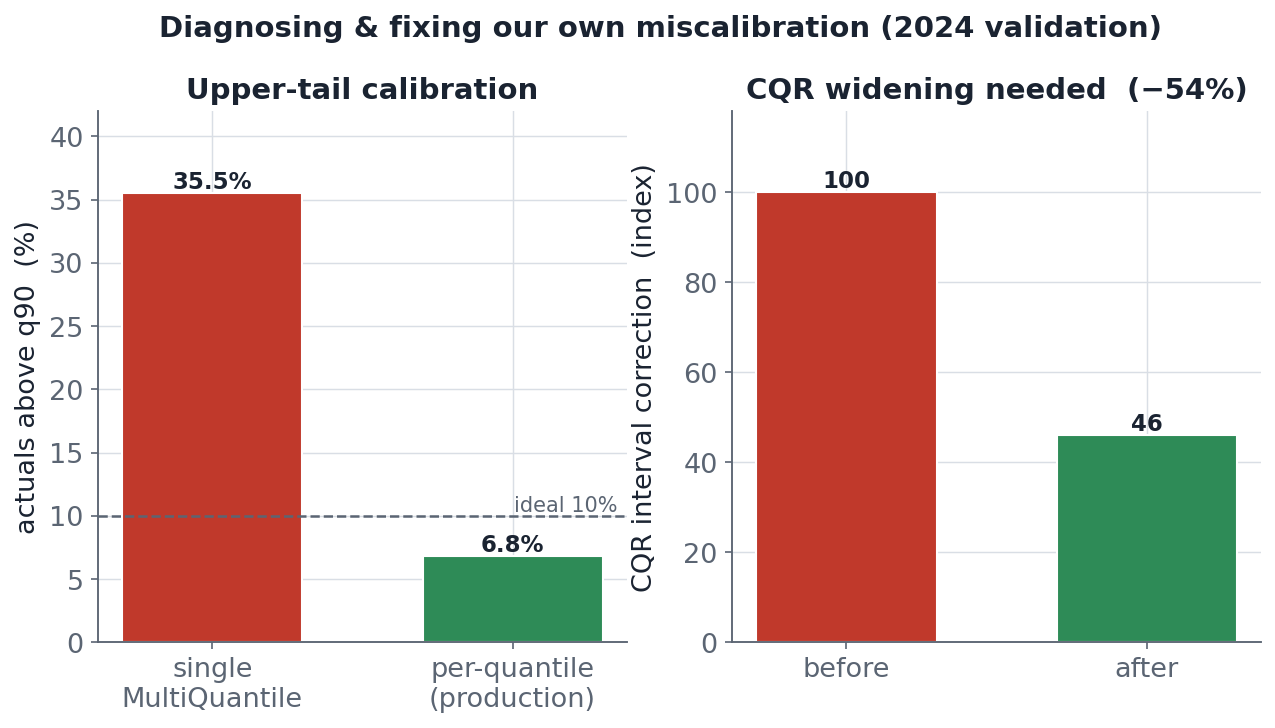
\includegraphics[width=\linewidth,height=0.66\textheight,keepaspectratio]{figures/module_b_calibration_fix.png}
    \end{column}
    \begin{column}{0.42\textwidth}
      \small
      We diagnosed our \emph{own} miscalibration: the upper tail was badly under-covered.
      \vspace{4pt}
      \begin{itemize}\setlength\itemsep{4pt}
        \item Per-quantile rewrite + CQR fixes it.
        \item CQR uses the $\big\lceil(n{+}1)(1{-}\alpha)\big\rceil/n$ quantile of calibration errors (finite-sample guarantee).
      \end{itemize}
    \end{column}
  \end{columns}
  \note{Rigor beat. Our first design under-covered the upper tail badly — 35.5\% of actuals
  above q90 (target 10\%). We found it, rewrote to per-quantile boosters, and added
  conformal calibration; the miss dropped to 6.8\%. Reporting your own bug and the fix
  builds credibility. ~45 s.}
\end{frame}

% =====================================================================================
% 13 — MODULE B RESULTS
% =====================================================================================
\begin{frame}{46\% better than seasonal-naive}
  \centering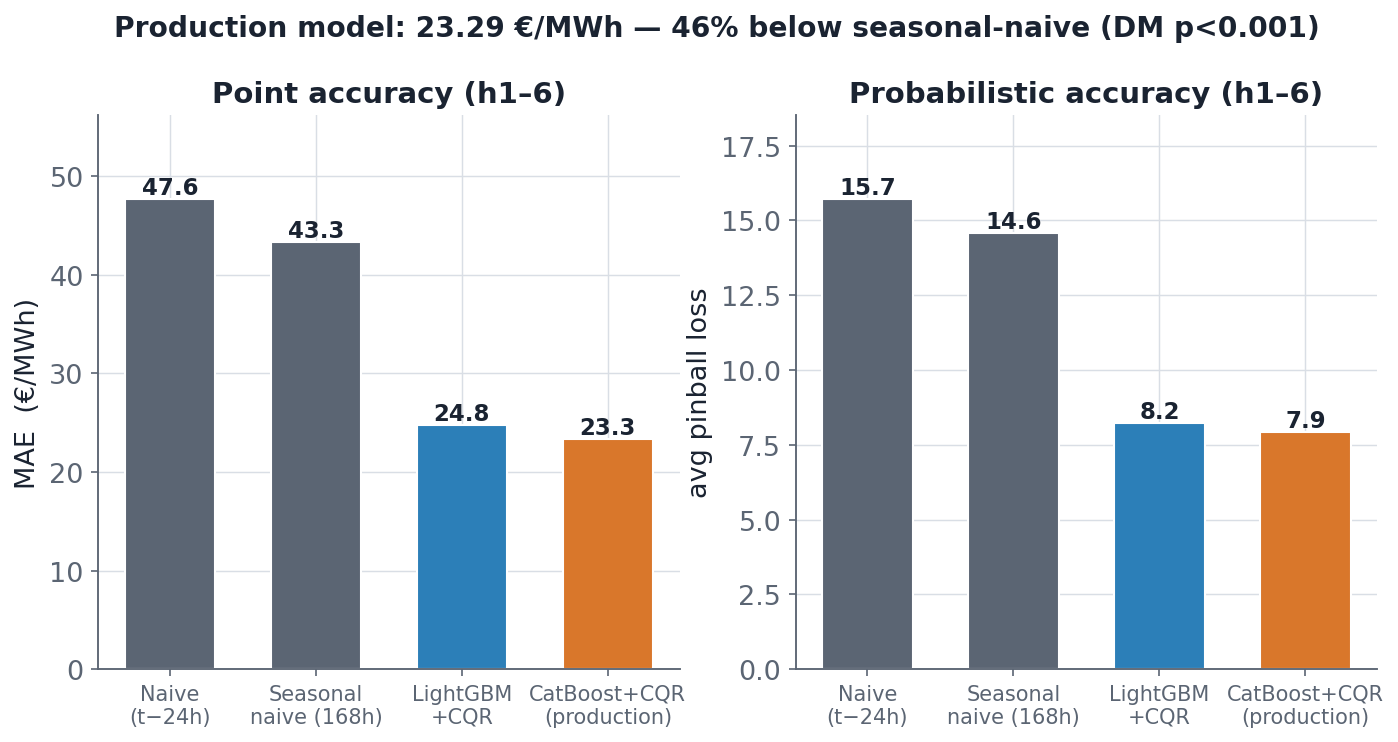
\includegraphics[width=\linewidth,height=0.66\textheight,keepaspectratio]{figures/module_b_leaderboard.png}
  \cap{Locked 2025-Q1 test, h1--6: MAE \textbf{23.29} \eur/MWh, pinball \textbf{7.93}, coverage \textbf{0.82}; Diebold--Mariano $p<0.001$.}
  \note{Headline result. On the locked Q1-2025 test set, CatBoost+CQR roughly halves the
  error of a strong seasonal-naive baseline, on both point and probabilistic metrics, and
  the gap is statistically significant. This is the production model that feeds Module C.
  ~55 s.}
\end{frame}

% =====================================================================================
% 14 — MODULE B HONEST NEGATIVE
% =====================================================================================
\begin{frame}{An honest negative: load did not help price}
  \vspace{0.3cm}
  \begin{columns}[T,onlytextwidth]
    \begin{column}{0.46\textwidth}
      \centering
      \colorbox{emisGrid!50}{\parbox[c][2.6cm][c]{0.9\linewidth}{\centering
        {\Large\bfseries\color{emisMuted} $\approx 0\%$}\\[4pt]
        {\small change in price MAE when Module A's load quantiles are added as features}}}
    \end{column}
    \begin{column}{0.50\textwidth}
      \small
      \begin{itemize}\setlength\itemsep{6pt}
        \item Wired A$\rightarrow$B, measured, found \textbf{no material gain}.
        \item We report the null result rather than hide it.
        \item Foreshadow: load \emph{will} help --- but later, at the dispatch stage.
      \end{itemize}
    \end{column}
  \end{columns}
  \note{Honesty beat. We tested whether load forecasts improve price forecasts. They
  don't — under 1\% change. We report it. Crucially this is not the end of Module A's
  story: it sets up the surprise that load DOES help the battery agent. ~40 s.}
\end{frame}

% =====================================================================================
% 15 — MODULE C ENV & REWARD
% =====================================================================================
\setact{Module C --- Dispatch}{modC}
\begin{frame}{Module C --- battery dispatch with CVaR-aware RL}
  \vspace{0.1cm}
  \centering
  \resizebox{0.96\textwidth}{!}{%
  \begin{tikzpicture}[node distance=8mm]
    \node[emisbox, draw=emisMuted, fill=emisGrid!50, text width=3.5cm] (obs)
      {Observation\\[1pt]\footnotesize SoC, calendar, last price,\\[-1pt] \textbf{B's q10/q50/q90} $\times$24h\\[-1pt] ($+$ \textbf{A's load} in B{+}A)};
    \node[emisbox, draw=modC, fill=modC!14, right=of obs] (pol) {RL policy\\PPO / SAC};
    \node[emisbox, draw=emisInk, fill=emisGrid!35, right=of pol] (act) {charge /\\discharge};
    \node[emisbox, draw=modB, fill=modB!12, right=of act] (bat) {Battery\\100 MWh};
    \draw[qarr, draw=emisMuted] (obs)--(pol);
    \draw[qarr, draw=modC] (pol)--(act);
    \draw[qarr, draw=emisInk] (act)--(bat);
    \draw[qarr, draw=modB] (bat.south) to[out=-90,in=-90] node[below,font=\scriptsize,text=emisMuted]{new state} (obs.south);
  \end{tikzpicture}}
  \vspace{0.30cm}

  $\displaystyle r_t \;=\; \underbrace{p_t\,a_t\,\Delta t}_{\text{step profit}}\;-\;\lambda\,\max\!\big(0,\,-\mathrm{CVaR}_{5\%}\big),\qquad \lambda = 0.1$

  \vspace{0.15cm}
  {\footnotesize\color{emisMuted} 100 MWh / 50 MW battery, 90\% round-trip efficiency, 24-h episodes.}
  \note{Module C. The agent sees its state of charge plus Module B's price fan --- and, in
  the B+A variant, Module A's load fan too --- and chooses to charge or discharge. Reward is
  profit minus a penalty on tail risk (CVaR), so it makes money without courting disaster.
  ~50 s.}
\end{frame}

% =====================================================================================
% 16 — MODULE C RESULTS
% =====================================================================================
\begin{frame}{SAC beats a perfect-foresight oracle}
  \centering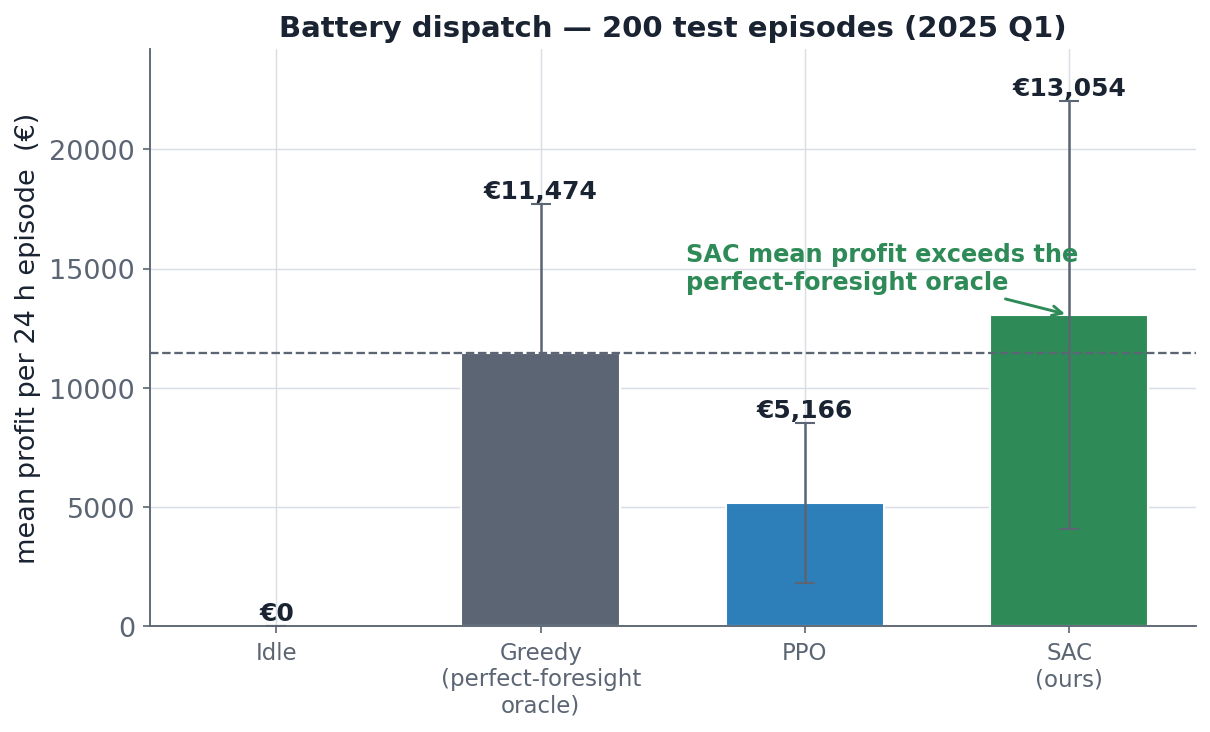
\includegraphics[width=\linewidth,height=0.66\textheight,keepaspectratio]{figures/module_c_profit.png}
  \cap{200 test episodes (2025 Q1): SAC mean \textbf{\eur13{,}054} vs.\ perfect-foresight oracle \textbf{\eur11{,}474} --- on forecasts alone.}
  \note{The payoff — pause here. SAC, which only sees forecasts, earns more on average
  than a greedy agent that is given the true future prices. That is the proof that a
  calibrated probabilistic forecast plus risk-aware RL can beat naive perfect-foresight
  trading. ~50 s.}
\end{frame}

% =====================================================================================
% 17 — MODULE C ABLATION
% =====================================================================================
\begin{frame}{Where each forecast earns its keep}
  \centering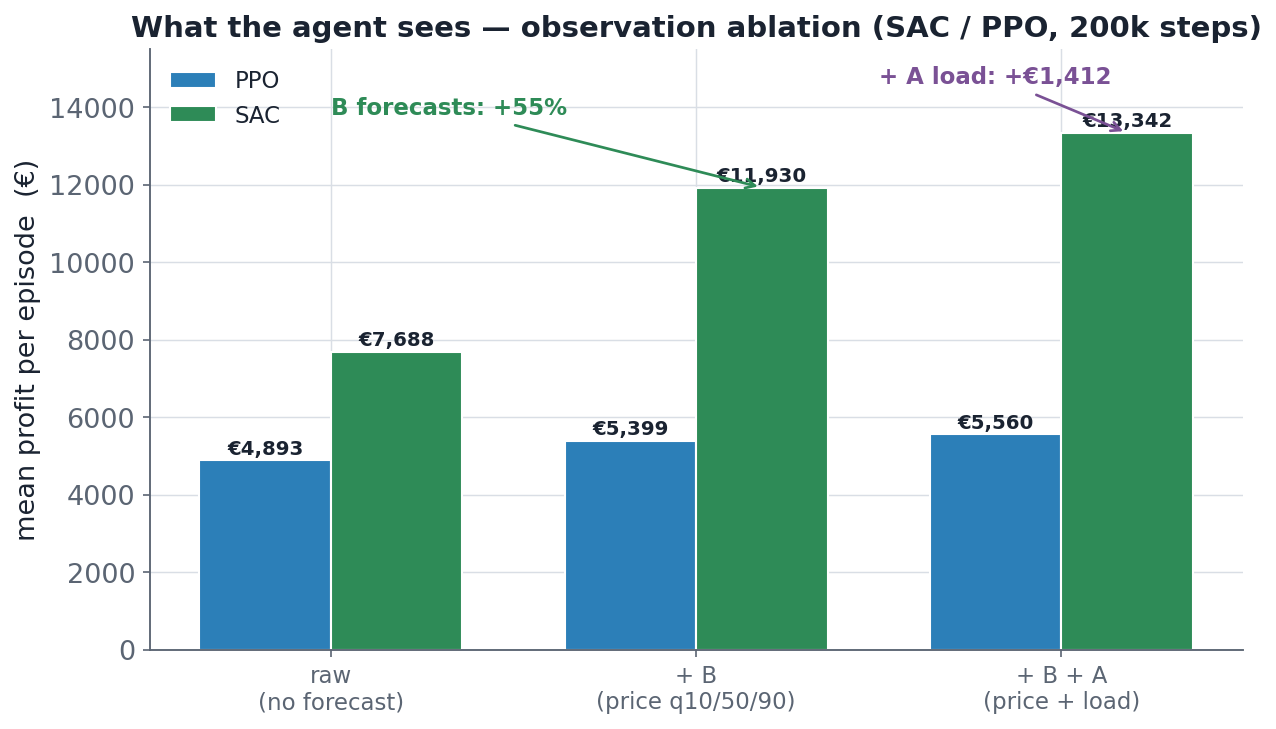
\includegraphics[width=\linewidth,height=0.66\textheight,keepaspectratio]{figures/module_c_ablation.png}
  \cap{Module B price forecasts: \textbf{+55\%} for SAC; adding Module A load \textbf{+\eur1{,}412} ($+$12\%) --- \textbf{A$\rightarrow$C helps}.}
  \note{Why it works. Stripping the forecasts collapses profit: price quantiles are worth
  +55\%. And here is the twist — Module A's load forecasts, which did NOT help price,
  DO help dispatch: another +12\% and a better Sharpe. Each forecast earns its place at
  the right stage. ~55 s.}
\end{frame}

% =====================================================================================
% 18 — CASCADE VALUE CHAIN
% =====================================================================================
\setact{Conclusions}{emisAccent}
\begin{frame}{Following the uncertainty through the pipeline}
  \vspace{0.3cm}
  \centering
  \resizebox{0.98\textwidth}{!}{%
  \begin{tikzpicture}[node distance=10mm]
    \node[emisbox, draw=emisAccent, fill=emisAccent!10] (data) {Data};
    \node[emisbox, draw=modImp, fill=modImp!12, right=of data] (sshb) {SSHB};
    \node[emisbox, draw=modA, fill=modA!12, above right=6mm and 16mm of sshb] (A) {Module A\\Load};
    \node[emisbox, draw=modB, fill=modB!14, below right=6mm and 16mm of sshb] (B) {Module B\\Price};
    \node[emisbox, draw=modC, fill=modC!14, right=46mm of sshb] (C) {Module C\\Dispatch};
    \draw[qarr, draw=emisAccent] (data)--(sshb);
    \draw[qarr, draw=emisMuted] (sshb)--(A);
    \draw[qarr, draw=emisMuted] (sshb)--(B);
    \draw[qarr, dashed, draw=emisMuted] (A) to[out=-25,in=155]
        node[sloped,above,font=\scriptsize\bfseries,text=emisMuted]{$\approx 0\%$} (B);
    \draw[qarr, draw=modB, line width=1.4pt] (B) to[out=0,in=-120]
        node[sloped,below,font=\scriptsize\bfseries,text=modB]{$+55\%$} (C);
    \draw[qarr, draw=modA, line width=1.4pt] (A) to[out=0,in=120]
        node[sloped,above,font=\scriptsize\bfseries,text=modA]{$+$\eur1{,}412} (C);
  \end{tikzpicture}}
  \vspace{0.3cm}
  \begin{center}{\footnotesize\color{emisMuted}
   Each link measured: load doesn't help \emph{price} (A$\to$B), but price \emph{and} load both help \emph{dispatch} (B$\to$C, A$\to$C).}\end{center}
  \note{Synthesis. We graded every link. A to B carries no signal — the honest null.
  But B to C is a huge +55\%, and A to C adds a further 1{,}412 euro. The uncertainty we
  propagated is exactly what created value where it matters. ~35 s.}
\end{frame}

% =====================================================================================
% 19 — LIMITATIONS
% =====================================================================================
\begin{frame}{What we don't claim}
  \vspace{0.2cm}
  \begin{itemize}\setlength\itemsep{10pt}
    \item \textbf{13 variables stay structurally red} --- data the API never recorded cannot be recovered.
    \item \textbf{Module A over-forecasts} the shifted 2025 winter (distribution drift).
    \item \textbf{SAC's higher mean carries fatter tail risk} (CVaR $<0$); the safer policy is PPO with B$+$A.
  \end{itemize}
  \note{Limitations — name them before the examiners do. Structural gaps are unfixable;
  2025 drifted from training; and SAC's extra profit comes with tail risk, so a
  risk-averse operator should prefer PPO with full features. ~25 s.}
\end{frame}

% =====================================================================================
% 20 — CONCLUSION
% =====================================================================================
\begin{frame}{Uncertainty, propagated, becomes profit}
  \vspace{0.25cm}
  \centering
  \statcard{modB}{23.29 \eur/MWh}{price MAE\\($-$46\% vs.\ seasonal-naive)}\hfill
  \statcard{modC}{\eur13{,}054}{SAC \emph{mean} profit / ep.\\(beats the oracle)}\hfill
  \statcard{modImp}{53.9\%}{cells repaired by SSHB\\(0 physical violations)}
  \vspace{0.5cm}

  \begin{center}\itshape\small
    Honest uncertainty --- quantified, calibrated, and propagated --- is what turns a
    battery into profit.
  \end{center}
  \vspace{0.25cm}
  {\footnotesize\color{emisMuted}\centering
   Rigor throughout: conformal calibration $\cdot$ gapped time-series CV $\cdot$ CVaR risk control $\cdot$ honest negatives $\cdot$ a locked test set.\par}
  \vspace{0.35cm}
  \begin{center}{\color{emisAccent}\bfseries Thank you --- questions welcome.}\end{center}
  \note{Close. Three numbers to remember: a 46\% better price forecast, a battery that
  beats the oracle, and an imputer that repairs half the missing cells without a single
  physical violation. Restate the through-line sentence, then open for questions. ~30 s.}
\end{frame}

% =====================================================================================
% BACKUP
% =====================================================================================
\setact{Appendix}{emisMuted}
\begin{frame}[allowframebreaks]{Appendix --- details}
  \footnotesize
  \textbf{Splits (fixed, locked test).}
  \begin{tabular}{@{}l l r@{}}
    \toprule
    split & period & hours\\\midrule
    train & 2019--2023 & 43{,}824\\
    val   & 2024 & 8{,}784\\
    test  & 2025 Q1 (locked) & 2{,}160\\
    \bottomrule
  \end{tabular}

  \medskip
  \textbf{Models.}
  \begin{itemize}\setlength\itemsep{2pt}
    \item Imputer: SAITS\,(Glocal-IB fork) --- 4 layers, $d_{\text{model}}{=}512$, 8 heads, FFN 1024; 168-h windows, stride 24; VIB (training) + SSHB (inference).
    \item Module A: dual-branch LSTM (48 h + 168 h) $\rightarrow$ MLP head; pinball loss; CQR.
    \item Module B: 3 CatBoost boosters, depth 8/6/8, $\ell_2$ 1/3/1; $\approx$33 causal features; CQR.
    \item Module C: PPO \& SAC (Stable-Baselines3); 78-dim observation; reward $=$ profit $-\,\lambda\,\max(0,-\mathrm{CVaR}_{5\%})$, $\lambda{=}0.1$.
  \end{itemize}

  \medskip
  \textbf{Validation.} Rolling-origin and expanding-window time-series CV, each with a
  \textbf{24-h gap} to prevent lag-24 leakage. The 2025-Q1 test set is touched only once.

  \framebreak
  \textbf{References \& tools.}
  \begin{itemize}\setlength\itemsep{3pt}
    \item Data: ENTSO-E Transparency Platform, Open-Meteo, Yahoo Finance / Energy-Charts.
    \item Imputation: SAITS (Du et al., 2023) / Glocal-IB.
    \item Forecasting: CatBoost; Conformal Quantile Regression (Romano et al., 2019; Barber et al., 2021).
    \item RL: PPO (Schulman et al., 2017), SAC (Haarnoja et al., 2018); CVaR (Rockafellar \& Uryasev, 2000).
    \item Libraries: PyTorch, PyPOTS, CatBoost, scikit-learn, Stable-Baselines3, Gymnasium, matplotlib.
  \end{itemize}
  \note{Backup slides for Q\&A: exact splits, model hyper-parameters, the gapped CV scheme,
  and references.}
\end{frame}

\end{document}
